\chapter{State of the art}
\label{chap:stateoftheart}

\drop{T}{his} chapter aims to explain the concepts and techniques in which
Alcaudon is based on. As shown in Figure ~\ref{fig:mindmap}. the project has foundations in
distributed systems, job scheduling, library design and data processing. In the
next subsections, those concepts will be analyzed in more depth.

\begin{figure}[!h]
\begin{center}
\includegraphics[width=1\textwidth]{mindmap.png}
\caption{Alcaudon foundations}
\label{fig:mindmap}
\end{center}
\end{figure}

\subsection{Data Processing}

According to a recent study by Cisco \cite{ciscosurvey}~\ref{fig:ciscodata} the
data storage is growing by 40\% yearly. That means that by 2020 datacenters will
store over 1000 ExaBytes of information. Keeping that data in silos without
performing any use of it is a poor investment.

\begin{figure}[!h]
\begin{center}
\includegraphics[width=0.8\textwidth]{ciscodata.png}
\caption{Actual Data Stored in Data Centers\cite{ciscosurvey}}
\label{fig:ciscodata}
\end{center}
\end{figure}

Processing those amounts of data using traditionals RDBMS is not practical, as they
are not designed to work with that much data. In the last years there have been
many ongoing efforts on providing tools to process and analyze large volumes of
data. Some examples could be MapReduce\cite{mapreduce}, Spark\cite{spark} and
many others. Before those frameworks appeared, there were some systems capable
of processing large amounts of data, like the supercomputers or HPC. One of the
main drawbacks of HPC is accessibility to those high end computers. Acquiring a
new Supercomputer in the event of a peak on data production is not feasible. For
companies, making an investment in a super computer is a big risk that in some
cases will not be reverted as profit.Another interesting point to make is that
Supercomputers perform well many floating-point operations per second. However,
in general the computations executed in systems like MapReduce are simple
strings manipulation, counting and so on. Given these usage patterns, it seems
that supercomputers are more suited to perform scientific analysis.

Once the limitations of HPC for \textit{big data} scenarios has been described
it is possible to explore how modern internet companies are using computing
resources to process data. For new organizations, it makes more sense to take
advantage of commodity hardware to process large amounts of data. One of the
reasons is that there are many tools to distribute data processing among large
clusters of commodity machines. Once that job is done, those machines can be
turned off or used for other purposes. Working with those systems provides
flexibility, both in resource usage and innovation capacity. 

\subsubsection{Cloud Computing}

The data processing systems described above fits very well with cloud computing
offerings such as IaaS providers.
During 2002 Amazon.com launched Amazon Web Services(AWS), one of the first cloud
providers. The idea behind AWS is to provide computing resources as a service, basically
outsourcing all the datacenter needs. The interesting part about AWS is that it provides
the needed elasticity 

\subsection{Distributed systems}
\label{subsection:distsys}

Distributed systems can be defined as a set of computer programs, executing on
one or more computers, and coordinating actions by exchanging \textit{messages}
\cite{GuideReliable}. Those computers are usually located in a \textit{computer
  network}, a collection of computers interconnected by hardware that supports
message passing and implement routing protocols. But if this definition is taken
to the extreme, a modern multi-core processor can be characterized as a
distributed system, with many components exchanging information in a network and
coordinating actions to get work done. To some extent, it's possible to see
distributed systems as a super set of concurrent systems.

A more common example of a distributed system it is a user requesting a web page to
a server with his smartphone. This example is a typical \textit{client-server}
model. This \textit{simple} action involves the interaction of various services
such as DNS servers, load balancers, HTTP proxies and HTTP servers. All these
services use a network as a mean to interchange messages as shown in figure
~\ref{fig:client-server}.

\begin{figure}[!h]
\begin{center}
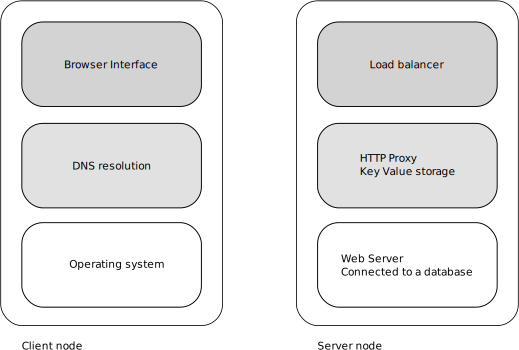
\includegraphics[width=0.7\textwidth]{client-server.png}
\caption{Client-server architecture}
\label{fig:client-server}
\end{center}
\end{figure}

As it has been previously discussed, distributed systems are very common
nowadays. They are present in fields like database systems, internet of things,
data processing and many more.

There are some reasons that make more convenient to work with distributed
systems, but the main reason is ability to scale. As defined in \cite{cloudadmin}
\begin{quote}
  A system's ability to scale is its ability to process a growing workload,
  usually measured in transactions per second, amount of data or number of
  users.
\end{quote}

Distributed programming can help designing systems with the ability to scale given
the following properties:

\begin{figure}[!h]
\begin{center}
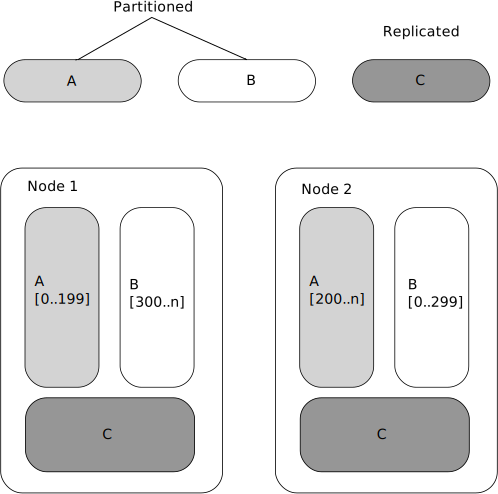
\includegraphics[width=0.7\textwidth]{partition-rep.png}
\caption{Partitioning and Replication}
\label{fig:partitioning}
\end{center}
\end{figure}

\begin{itemize}
\item \textit{Reliability}: Achieved by \textit{replication} and/or
  \textit{partitioning} as illustrated in Figure ~\ref{fig:partitioning}.
\item \textit{Elasticity}: Since the systems are designed to work in
  coordination with other processes, it is possible to add more resources to
  handle increasing workloads. But there is an upper limit imposed by the
  coordination model used.
\item \textit{Parallelism}: This is a natural outcome of having multiple resources, they
  can get work done in parallel.
\item \textit{Price/performance ratio}: Scaling vertically (using more powerful
  compute nodes), has upper limits both in available technology and in costs. As
  shown in Figure ~\ref{fig:highend} the performance gap between a high end
  server and a cluster of commodity hardware nodes is tolerable. Another factor
  to take into account when distributed systems are used is the cost of
  networking communications, as it implies an overhead in the computations.
\end{itemize}

\begin{figure}[!h]
\begin{center}
\includegraphics[width=1\textwidth]{scalingcost.png}
\caption{Performance advantage of a cluster built with large SMP server nodes
  (128-core SMP) over a cluster with the same number of processor cores built
  with low-end server nodes (four-core SMP), for clusters of varying
  size.\cite{Datacenter}}
\label{fig:highend}
\end{center}
\end{figure}


\subsubsection{Taxonomy of a distributed system}

Once described what distributed systems are and why are useful, it is possible
to define a taxonomy of distributed systems topics such as coordination
algorithms, global state collection, distributed consensus, etc.

As it can be seen the topic is wide, so for this documents only
\textit{distributed snapshots}, \textit{membership protocols} and \textit{time
  in distributed systems} will be covered.

\begin{itemize}
\item Distributed snapshots: 
  Since Alcaudon aims to be a fault-tolerant system, guarantees about persistent
  state must be enforced. To design a resilient system, persistent state snapshots
  should be taken.
\item Time in distributed systems:

\item Membership protocols
\end{itemize}

\subsubsection{Distributed system reliability}

Building distributed systems is not an easy task. In this subsection, different
failure scenarios that can happen in a distributed environment will be presented.

As proposed by \cite{GuideReliable}, it is possible to classify system error
causes as follows:
\begin{itemize}
\item \textit{Hardware failures}: These kind of failures are inevitable, since
  hardware have a life cycle and some components might fail.
\item \textit{Software failures}: Bugs are quite common
\item Complexity
\item Lack of failure detection
\item Hostile environments
\end{itemize}

There are costs associated with distributed programming; network latency,
fault-tolerance mechanisms and consensus can have impact in the throughput
achieved by a system. In \cite{189908} a metric named Configuration that
Outperforms a Single Thread (COST), is proposed. It measures the number of cores
needed to outperform a single threaded implementation. In this experiments,
there are many distributed processing frameworks that don't perform properly
when they are compared to a single node implementations. As a conclusion, there
are scenarios where the costs associated with distributed computing are higher
than the gains.

Alcaudon goal is to provide users a simple but powerful interface that enables
them to parallelize and distribute computations for unbounded datasets without all
the described problems.

\subsubsection{Actor Model}

To tackle all the complexity described in previous section there is a
computation model that is well suited: the actor model.

The actor model provides a high level abstraction to deal with concurrent and
distributed systems. The theoretical model was developed by Carl Hewitt in
the seventies, but it was popularized by Erlang programming language\cite{erlang}
developed by Ericsson.

It can be characterized as follows:
\begin{itemize}
\item Actors communicate via asynchronous messages
\item Actors manage their state
\item In the event of a message response they can:
  \begin{itemize}
  \item Create new child actors
  \item Send messages to another actors
  \item Stop actors (even themselves)
  \item Change their behaviour for the next messages
  \end{itemize}
\end{itemize}

TODO add more info about akka.

\subsection{Job scheduling}

Talk about NP-Problem and some state of the art schedulers.

\subsection{Library design}
